\subsection{The Complex Plane}

\begin{tcolorbox}[title=Problem 3, breakable]
    Let $z$ be a complex number $\ne 0$. What is the absolute value of $z \sqrt{z}$?
\end{tcolorbox}

\textbf{Solution:} Let $z = x + yi$. 
\[
|z \sqrt{z}| = |z| \, |\sqrt{z}| = (x^2 + y^2)^{1/2} \cdot (x^2 + y^2)^{1/4} = (x^2 + y^2)^{3/4} = (z \overline{z})^{3/4} = (|z|^2)^{3/4} = |z|^{3/2}
\]

\begin{tcolorbox}[title=Problem 4, breakable]
    Prove the statements of Theorem $1$.
\end{tcolorbox}

\begin{enumerate}
    \item $\overline{zw} = \overline{z} \overline{w}$
    \item $\overline{z + w} = \overline{z} + \overline{w}$
    \item $\overline{\overline{z}} = z$
\end{enumerate}

\begin{proof}
    Let $z = x + yi$ and $w = u + vi$. Then
    \[
    zw = (x + yi)(u + vi) = (xu - yv) + (xv + yu)i, \quad \overline{zw} = (xu - yv) - (xv + yu)i
    \]
    and
    \[
    \overline{z} \, \overline{w} = (x - yi)(u - vi) = (xu - yv) - (xv + yu)i.
    \]
    Therefore $\overline{zw} = \overline{z} \, \overline{w}$.
    \[
    z + w = (x+u) + (y+v)i, \quad \overline{z + w} = (x+u) - (y+v)i = (x - yi) + (u - vi) = \overline{z} + \overline{w}.
    \]
    \[
    \overline{\overline{z}} = \overline{x - yi} = x + yi = z.
    \]
\end{proof}


\begin{tcolorbox}[title=Problem 5, breakable]
    Show that for any complex number $z = x + iy$, with $x, y$ real, we have 
    \[Im(z) \le |Im(z)| \le |z|\]
\end{tcolorbox}

\begin{proof}
    Notice
    \[
    \operatorname{Im}(z) = y.
    \]
    By definition of absolute value
    \[
    y \le |y| = |\operatorname{Im}(z)|.
    \]
    Then
    \[
    |\operatorname{Im}(z)| = |y| \le \sqrt{x^2 + y^2} = |z|.
    \]
    Combining these inequalities shows
    \[
    \operatorname{Im}(z) \le |\operatorname{Im}(z)| \le |z|.
    \]
\end{proof}

\subsection{Polar Form}

\begin{tcolorbox}[title=Problem 3, breakable]
    Let $z$ be a complex number $ \ne 0$.
    Show that there are precisely two distinct complex numbers 
        whose square is $z$.
\end{tcolorbox}

\begin{proof}
    We first show existence of two complex numbers whose square are $z$.
    Let $z = r e^{\theta i}$ where $\theta, r \in \mathbb{R}$
        and $0 \le \theta < 2 \pi$.
    Consider $\sqrt{r} e^{\theta/2 i}$. Notice 
    \[\sqrt{r} e^{\theta/2 i} \cdot \sqrt{r} e^{\theta/2 i} = r e^{\theta i}\]
    Now consider $-\sqrt{r} e^{\theta/2 i}$. Since $z \ne 0$, $\sqrt{r} \ne -\sqrt{r}$. Then 
    \[-\sqrt{r} e^{\theta/2 i} \cdot -\sqrt{r} e^{\theta/2 i} = r e^{\theta i}\]

    We now show these are the only two complex numbers whose square are $z$.
    Suppose $w$ is a complex number such that $w^2 = z = r e^{\theta i}$.
    Let $w = \rho e^{x i}$. Then
    \[
        w^2 = \rho^2 e^{2xi} = r e^{\theta i}
    \]
    Matching moduli shows $\rho = \sqrt{r}$.
    Matching arguments shows $2x = \theta + 2\pi k$ for some $k \in \mathbb{Z}$.
    Thus $x = \theta/2 + k\pi$.
    Since angles differing by $2\pi$ give the same complex number, only
    $k = 0, 1$ produce distinct values. These are exactly
    $\sqrt{r}e^{\theta i/2}$ and $-\sqrt{r}e^{\theta i/2}$.
\end{proof}

\begin{tcolorbox}[title=Problem 4, breakable]
    Let $z$ be a complex number $\ne 0$.
    Let $n$ be a positive integer.
    Show that there are $n$ distinct complex numbers $w$
        such that $w^n = z$.
    Write these complex numbers in polar form.
    The proof given that a polynomial of degree $\le n$
        has at most $n$ roots applies to the complex case,
        and thus we see that there are no other complex 
        numbers $w$ such that $w^n = z$ other than those 
        you have presumably written down.
\end{tcolorbox}

\begin{proof}
    We first show existence of $n$ complex numbers whose $n$-th power is $z$.  
    Let $z = r e^{\theta i}$ where $r, \theta \in \mathbb{R}$ and $0 \le \theta < 2\pi$.  
    Consider 
    \[
    w = r^{1/n} e^{(\theta + 2\pi k)i/n}, \quad k = 0, 1, \dots, n-1.
    \]  
    Notice that
    \[
    w^n = \bigl(r^{1/n} e^{(\theta + 2\pi k)i/n}\bigr)^n = r e^{\theta i} = z.
    \]  
    Since $k$ ranges from $0$ to $n-1$, these are $n$ distinct numbers.

    We now show that these are the only complex numbers whose $n$-th power is $z$.  
    Suppose $w$ is a complex number such that $w^n = z = r e^{\theta i}$.  
    Let $w = \rho e^{\phi i}$. Then
    \[
    w^n = \rho^n e^{n\phi i} = r e^{\theta i}.
    \]  
    Matching moduli gives $\rho = r^{1/n}$.  
    Matching arguments gives $n\phi = \theta + 2\pi k$ for some $k \in \mathbb{Z}$, so
    \[
    \phi = \frac{\theta + 2\pi k}{n}.
    \]  
    Angles differing by $2\pi$ give the same complex number, so only $k = 0, 1, \dots, n-1$ produce distinct values. These are exactly
    \[
    w = r^{1/n} e^{(\theta + 2\pi k)i/n}, \quad k = 0, 1, \dots, n-1.
    \]
\end{proof}

\begin{tcolorbox}[title=Problem 5, breakable]
    Write in polar form the $n$ complex numbers $w$ 
        such that $w^n = 1$. Plot all of these as points in the 
        plane $n = 2, 3, 4, 5$.
\end{tcolorbox}

\begin{center}
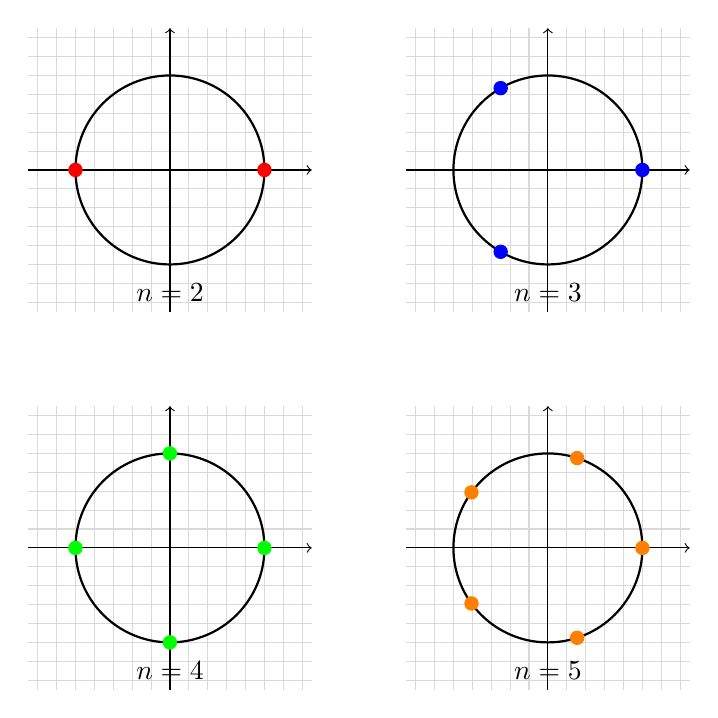
\begin{tikzpicture}[scale=1.2]
    % n = 2
    \begin{scope}[xshift=0cm, yshift=0cm]
    \draw[gray!30, step=0.2] (-1.5,-1.5) grid (1.5,1.5);
    \draw[->] (-1.5,0) -- (1.5,0);
    \draw[->] (0,-1.5) -- (0,1.5);
    \draw[thick] (0,0) circle(1);
    \foreach \k in {0,1} {
        \filldraw[red] ({cos(360*\k/2)}, {sin(360*\k/2)}) circle(2pt);
    }
    \node at (0,-1.3) {$n=2$};
    \end{scope}

    % n = 3
    \begin{scope}[xshift=4cm, yshift=0cm]
    \draw[gray!30, step=0.2] (-1.5,-1.5) grid (1.5,1.5);
    \draw[->] (-1.5,0) -- (1.5,0);
    \draw[->] (0,-1.5) -- (0,1.5);
    \draw[thick] (0,0) circle(1);
    \foreach \k in {0,1,2} {
        \filldraw[blue] ({cos(360*\k/3)}, {sin(360*\k/3)}) circle(2pt);
    }
    \node at (0,-1.3) {$n=3$};
    \end{scope}

    % n = 4
    \begin{scope}[xshift=0cm, yshift=-4cm]
    \draw[gray!30, step=0.2] (-1.5,-1.5) grid (1.5,1.5);
    \draw[->] (-1.5,0) -- (1.5,0);
    \draw[->] (0,-1.5) -- (0,1.5);
    \draw[thick] (0,0) circle(1);
    \foreach \k in {0,1,2,3} {
        \filldraw[green] ({cos(360*\k/4)}, {sin(360*\k/4)}) circle(2pt);
    }
    \node at (0,-1.3) {$n=4$};
    \end{scope}

    % n = 5
    \begin{scope}[xshift=4cm, yshift=-4cm]
    \draw[gray!30, step=0.2] (-1.5,-1.5) grid (1.5,1.5);
    \draw[->] (-1.5,0) -- (1.5,0);
    \draw[->] (0,-1.5) -- (0,1.5);
    \draw[thick] (0,0) circle(1);
    \foreach \k in {0,1,2,3,4} {
        \filldraw[orange] ({cos(360*\k/5)}, {sin(360*\k/5)}) circle(2pt);
    }
    \node at (0,-1.3) {$n=5$};
    \end{scope}
\end{tikzpicture}
\end{center}

\begin{tcolorbox}[title=Problem 6, breakable]
    If $\theta$ is real, show that 
    \[\cos \theta = \frac{e^{i \theta} + e^{-i \theta}}{2} \text{ and } \sin \theta = \frac{e^{i \theta} - e^{-i \theta}}{2i}\]
\end{tcolorbox}

\begin{proof}
    \begin{align*}
        \frac{e^{i \theta} + e^{-i \theta}}{2} 
            &= \frac{(\cos \theta + i \sin \theta) + (\cos(-\theta) + i \sin(-\theta))}{2} \\
            &= \frac{(\cos \theta + i \sin \theta) + (\cos \theta - i \sin \theta)}{2} \\
            &= \frac{2 \cos \theta}{2} \\
            &= \cos \theta
    \end{align*}
\end{proof}

\begin{proof}
    \begin{align*}
        \frac{e^{i \theta} - e^{-i \theta}}{2i} 
            &= \frac{(\cos \theta + i \sin \theta) - (\cos(-\theta) + i \sin(-\theta))}{2i} \\
            &= \frac{(\cos \theta + i \sin \theta) - (\cos \theta - i \sin \theta)}{2i} \\
            &= \frac{2 i \sin \theta}{2i} \\
            &= \sin \theta
    \end{align*}
\end{proof}